%\setcounter{paragraph}{1}
% Ejercicio 2 - a)
\paragraph{}\label{subsubsec:ej2-a}
Completar las entradas necesarias en la IDT para asociar diferentes rutinas a
todas las excepciones del procesador. Cada rutina de excepción debe indicar en
pantalla qué problema se produjo e interrumpir la ejecución. Posteriormente se
modificarán estas rutinas para que se continúe la ejecución, resolviendo el
problema y desalojando a la tarea que lo produjo.
\hruler

La IDT - $Interrupt$ $Descriptor$ $Table$ - es una tabla de descriptores de manejadores de interrupción. Cada entrada describe la atención de
un tipo de interrupción en particular. Tiene la siguiente forma:

\begin{figure}[H]
\begin{center}
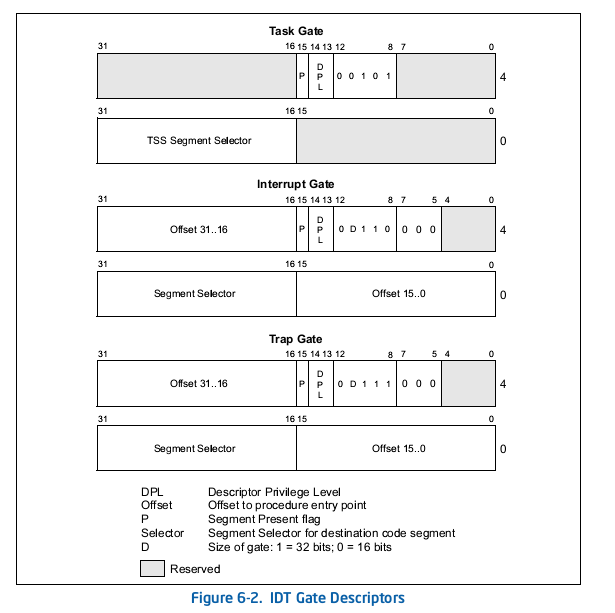
\includegraphics[]{imagenes/idt_entry.png}
\end{center}
\end{figure}

Nosotros vamos a usar descriptores del tipo $Interrupt gate$.

En éste ejercicio vamos a ocuparnos de las excepciones del procesador, cuyo tipo va entre 0 y 19.
Para cada una nuestra rutina de atención será imprimir los detalles de la excepción, según el manual de Intel. Más adelante vamos a tener que
desalojar a la tarea donde se produce la excepción, y además guardar los detalles de la excepción para poder mostrarla en pantalla cuando
el usuario presiona las teclas de 1 a 8.
Con tal propósito llenamos las entradas de la IDT de la siguiente forma.

\begin{itemize}
    \item segment-selector = 0x40 (de código de nivel 0)
    \item offset = la dirección donde escribimos la rutina de tal excepción
    \item p = 1 (presente)
    \item dpl = 0 (nivel administrador) \fixme{solo puede llamarlas m?, o es que las llama el procesador}
    \item d = 1 (32 bits)
\end{itemize}

% Ejercicio 2 - b)
\paragraph{}\label{subsubsec:ej2-b}
Hacer lo necesario para que el procesador utilice la IDT creada anteriormente.
Generar una excepción para probarla.

Nota: La IDT es un arreglo de idt entry declarado solo una vez como idt. El
descriptor de la IDT en el código se llama IDT DESC. Para inicializar la IDT se
debe invocar la función idt inicializar.
\hruler
Debemos cargar el descriptor de nuestra IDT, llamado IDT\_DESC, con la instrucción especial $lidt$. 

Una excepción interesante que utilizamos fue dividir por cero, que hizo saltar la excepción número 0.
